\appendix
\renewcommand{\listtablename}{Anhang}
\renewcommand{\lstlistingname}{} 
\renewcommand{\thelstlisting}{Quellcode \arabic{lstlisting}}
\listoftables
\refstepcounter{section}
\definecolor{BackgroundColor}{RGB}{225,225,225,225}	
\lstset{backgroundcolor=\color{BackgroundColor}, numbers=left, frame=single}

%%% Beginn	
	\newpage	
	\subsection{Initialisierungsfunktion}
	\label{a1}
	\addcontentsline{lot}{section}{A.1 Initialisierungsfunktion}	
	\begin{figure}[h!]
	\centering
		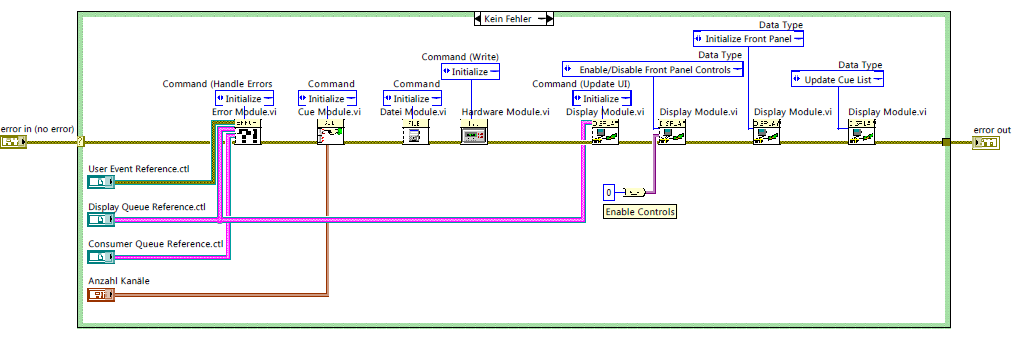
\includegraphics[angle=90, height=0.8\textheight ]{Pics/init.png}
	\caption{Initialisierungsfunktion}
	\label{fig:a1}
	\end{figure}
	\newpage
	
	\subsection{Shutdown-Funktion}
	\addcontentsline{lot}{section}{A.2 Shutdown-Funktion}
	\begin{figure}[h!]
	\centering
		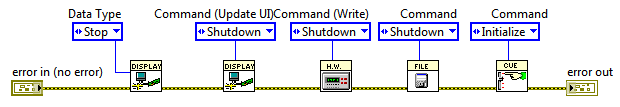
\includegraphics[width=\textwidth]{Pics/shutdown.png}
	\caption{Shutdown-Funktion}
	\label{fig:a2}
	\end{figure}
	%\newpage
	


	\subsection{Initialisierung des Front Panels}
	\addcontentsline{lot}{section}{A.3 Initialisierung des Front Panels}	
	\begin{figure}[h!]
	\centering
		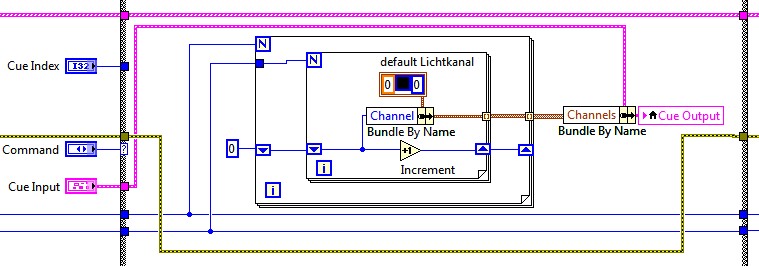
\includegraphics[width=\textwidth]{Pics/init-front.png}
	\caption{Initialisierung des Front Panels}
	\label{fig:a3}
	\end{figure}
	%\newpage
	


	\subsection{Auswahl eines Lichtsets aus der Lichterset Queue}
	\addcontentsline{lot}{section}{A.4 Auswahl eines Lichtsets aus der Lichterset Queue}	
	\begin{figure}[h!]
	\centering
		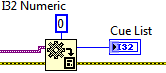
\includegraphics[width=0.5\textwidth]{Pics/front-auswahl.png}
	\caption{Auswahl eines Lichtsets aus der Lichterset Queue}
	\label{fig:a4}
	\end{figure}
	%\newpage
	
	\subsection{De-/Aktivieren von Schaltflächen}	
	\addcontentsline{lot}{section}{A.5 De-/Aktivieren von Schaltflächen}	
	\begin{figure}[h!]
	\centering
		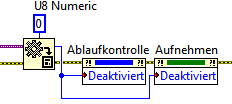
\includegraphics[width=0.5\textwidth]{Pics/front-deaktivieren.png}
	\caption{De-/Aktivieren von Schaltflächen}
	\label{fig:a5}
	\end{figure}
	%\newpage

	\subsection{Update der Set-Ablaufliste}
	\addcontentsline{lot}{section}{A.6 Update der Set-Ablaufliste}
	\begin{figure}[h!]
	\centering
		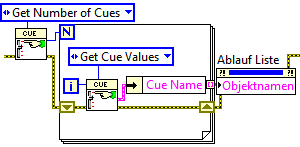
\includegraphics[width=0.5\textwidth]{Pics/front-updateCue.png}
	\caption{Update der Set-Ablaufliste}
	\label{fig:a6}
	\end{figure}
	%\newpage	
	
	

	\subsection{Update der Lichtkanäle}
	\addcontentsline{lot}{section}{A.7 Update der Lichtkanäle}	
	\begin{figure}[h!]
	\centering
		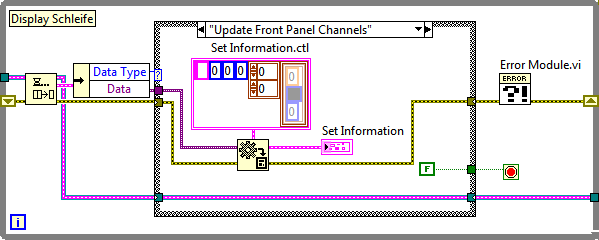
\includegraphics[width=0.5\textwidth]{Pics/front-kanale.png}
	\caption{Update der Lichtkanäle}
	\label{fig:a7}
	\end{figure}
	%\newpage	
	
	\subsection{Timing Modul}
	\addcontentsline{lot}{section}{A.8 Timing Modul}	
	\begin{figure}[h!]
	\centering
		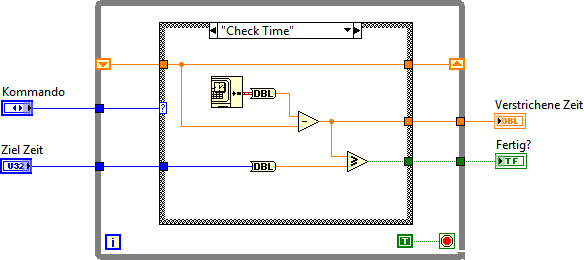
\includegraphics[width=0.5\textwidth]{Pics/zeit.png}
	\caption{Timing Modul}
	\label{fig:a8}
	\end{figure}
	%\newpage	
	
	\subsection{Text}
	\addcontentsline{lot}{section}{A.9 Text}	
	\begin{figure}[h!]
	\centering
		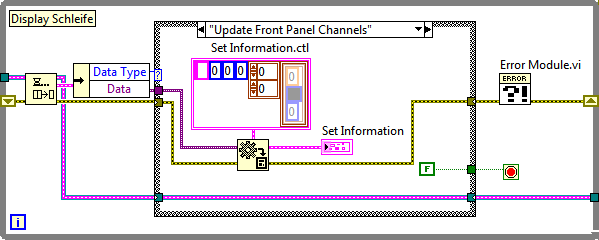
\includegraphics[width=0.5\textwidth]{Pics/front-kanale.png}
	\caption{Text}
	\label{fig:a9}
	\end{figure}
	%\newpage	
	
	\subsection{Text}
	\addcontentsline{lot}{section}{A.10 Text}	
	\begin{figure}[h!]
	\centering
		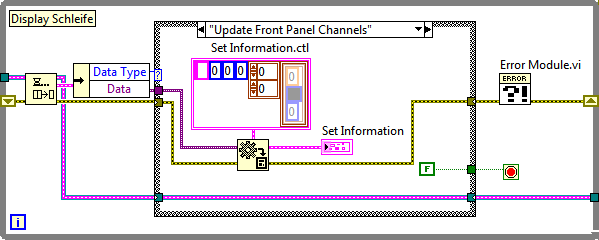
\includegraphics[width=0.5\textwidth]{Pics/front-kanale.png}
	\caption{Text}
	\label{fig:a10}
	\end{figure}
	%\newpage	
	
	\subsection{Text}
	\addcontentsline{lot}{section}{A.11 Text}	
	\begin{figure}[h!]
	\centering
		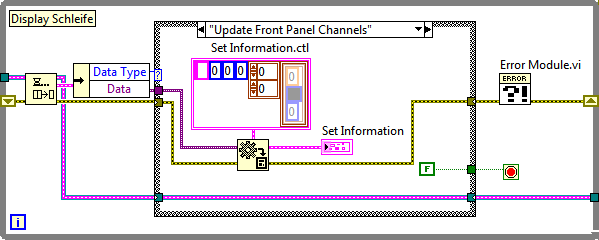
\includegraphics[width=0.5\textwidth]{Pics/front-kanale.png}
	\caption{Text}
	\label{fig:a11}
	\end{figure}
	%\newpage	
	
